%!TEX root=../book.tex

\chapter{\textit{t}-Tools}

\section{Overview of \textit{t}-Tools}

\subsection{One-Sample \textit{t}-Test}

The one-sample \textit{t}-test is one of the simplest entry points to inferential statistics there is. Simply put, it seeks to determine if the average value of a set of data differs significantly from some theoretical quantity. Say, for instance, we are working in a lumber mill and it looks like a shipment of Douglas fir trees is a bit smaller than usual. We know that a typical Douglas fir from this region is about 225 feet tall and has a radius of 7.5 feet, giving us a total volume of about $39000$ cubic feet.

So we take the measurements for each of the trees in this shipment and find that the average volume is $36500$ cubic feet with a standard deviation around $\sigma = 2000$ cubic feet. Do we have sufficient proof that these trees are actually smaller than our typical shipment?

Well, unfortunately, the human brain isn't great at intuitively figuring out if differences like that are meaningful or within the expected margin of error: that's where inferential statistics come into play. So let's first state our hypotheses as:
\begin{eqnarray*}
H_0:& \bar{x} = \mu\\
H_A:& \bar{x} \neq \mu
\end{eqnarray*}
where $\bar{x}$ is the mean volume of our shipment of trees and $\mu$ is the mean volume of adult Douglas firs. Now, we can conduct our statistical test.

A \textit{t}-test, speaking generally, takes the form:
\begin{equation}
t = \frac{\text{Estimate}-\text{Parameter}}{SE(\text{Estimate})}
\end{equation}
The specifics of what you plug in for the estimate and the parameter will vary a bit depending on which type of \textit{t}-test you use; however, they all are based off of this.

In our case, the one-sample \textit{t}-test will look like:
\begin{equation}
t=\frac{\bar{x}-\mu}{s_x}
\end{equation}
where each of the variables is what we defined in our hypotheses above. Plugging in our data we get:
\begin{eqnarray*}
t(124)&=&\frac{36500-39000}{2000/\sqrt{125}} \\
&=& -13.98
\end{eqnarray*}
Although we have our standardized \textit{t}-statistic, we still don't know if it reaches a level of significance or not. historically, we would have to go to a table of \textit{p}-values and look up the one that was closest to our \textit{t}-statistic given the degrees of freedom (here, 124, or $n-1$). Thankfully, we now have software that is able to compute this value for us much more precisely and quickly. In this case, we end up with a \textit{p}-value $< 0.001$, showing that the result is highly significant.

\begin{figure}[h]
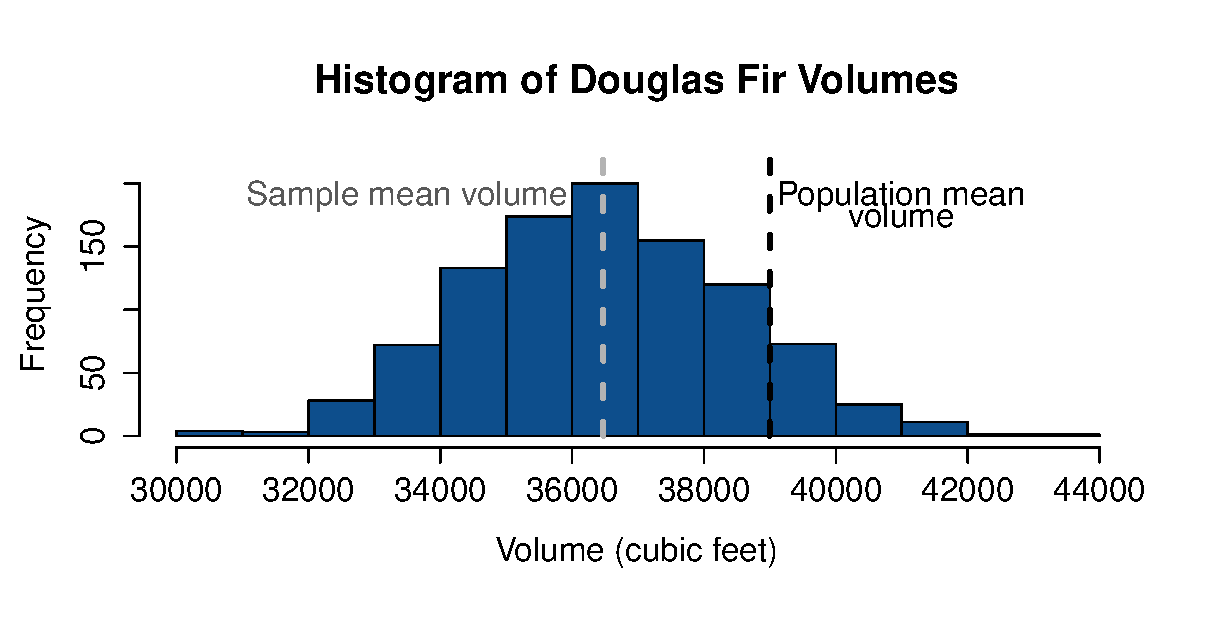
\includegraphics[width=35pc]{t01}
\label{fig:t01}
\caption{Histogram of the volumes of a shipment of Douglas firs with mean volume $36500$ cubic feet and standard deviation $\sigma = 2000$ cubic feet. A one-sample \textit{t}-test shows that this shipment of firs is significantly smaller than the typical shipment (mean $39000$ cubic feet), $t=-13.98$, $p\text{-value}<0.001$.}
\end{figure}

Moreover, we can infer the direction of this difference. Remember that the \textit{t}-statistic is computed by subtracting our estimated mean from our population mean: given this, a negative \textit{t}-statistic means that the sample mean is less than the population mean whereas a positive \textit{t}-statistic shows that our sample mean is greater than that of the population.

So, we can ultimately conclude that this shipment of Douglas firs is statistically significantly below the average size of a shipment, given $t(124)=-13.98$ with a $p\text{-value} < 0.001$. We can summarize this difference in Figure \ref{fig:t01}.

\subsection{Paired-Samples \textit{t}-Test}

So now that we're familiar with a one-sample \textit{t}-test, the next two tests in the suite become really easy to understand. In a one-sample \textit{t}-test, we're testing one sample of data against a mean that we already know; with a paired-samples test, we extend that to two samples of data that are usually matched along some criteria. For instance, we might be looking at the difference in grieving patterns between mothers and fathers; or personality differences between heterozygous twins; or blood pressure of clinic patients before and after a given drug treatment.

In every case, our two variables are somehow \textit{related} to one another and for every data point in column A there is a corresponding data point in column B. For instance, let's say that we work at a large health clinic and we're testing a new drug, Procardia, that's meant to reduce hypertension. We find 1000 individuals with a high systolic blood pressure ($M=145$mmHg, $SD=9$), we give them Procardia for a month, and then measure their blood pressure again. We find that the mean systolic blood pressure has decreased to $138$mmHg with a standard deviation $8$. We can visualize this difference in Figure \ref{fig:t02}.

\begin{figure}[h]
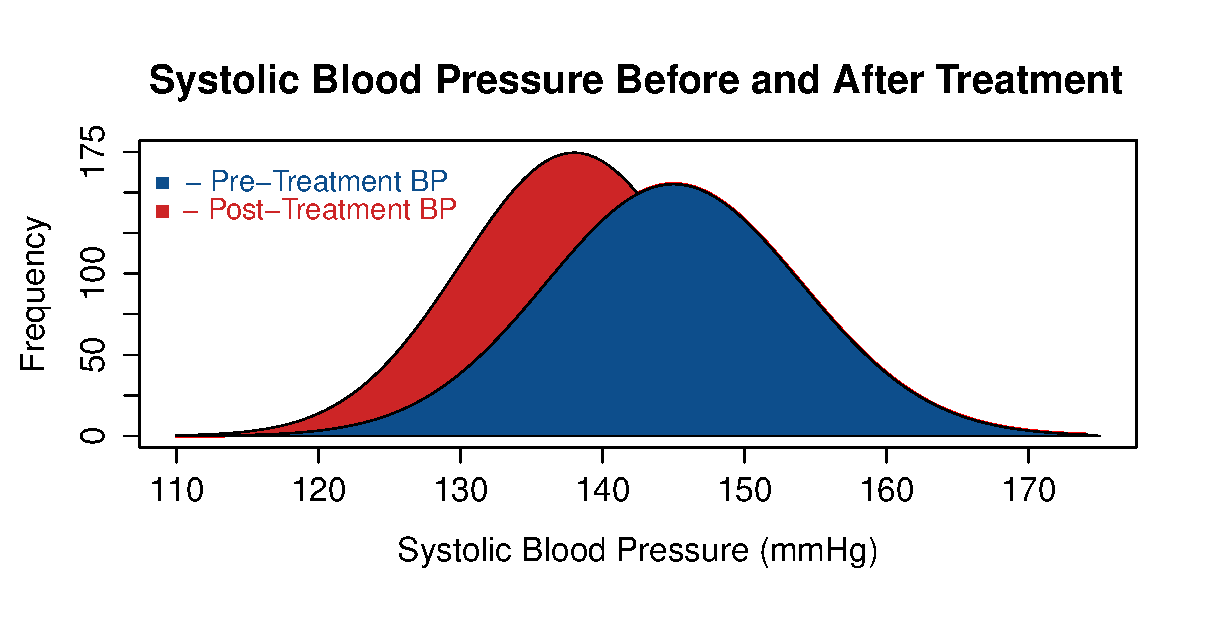
\includegraphics[width=35pc]{t02}
\label{fig:t02}
\caption{Systolic blood pressures before and after treatment with an antihypertensive drug.}
\end{figure}

So, we know that these data are paired: we used the same individuals for both pre-treatment and post-treatment and there are 1000 observations for each column of data. We know that the pre-treatment and post-treatment mean systolic blood pressures are different, but we want to know if this difference is statistically significant. In this case, our \textit{t}-test will take the form:
\begin{equation}
t=\frac{\bar{x}_1-\bar{x}_2}{s_{x_1-x_2}}\text{, where }s_{x_1-x_2}=\sqrt{\frac{s_1^2}{n_1}+\frac{s_2^2}{n_2}}
\end{equation}
Plugging in our data, we end up with $t(999)=19.75$, $p\text{-value}<0.001$, indicating that (yay!) our experimental drug does appear to actually reduce hypertension in individuals!

\subsection{Independent-Samples \textit{t}-Test}

Finally is the independent-samples \textit{t}-test. Functionally, this is nearly identical to the paired-samples test: the only major difference is that it is used when the two samples are not paired or somehow related to one another. We would use this test if we were interested in determining, for example, whether there was a difference between depression scores of outpatients at two different clinics; or whether New Yorkers and Clevelanders spend different amounts of money each month eating out; or do two strains of a bacteria respond differently to an antimicrobial gel?

In each of these examples, there is no pairing: New Yorkers are an entirely different population from Clevelanders; the two strains of bacteria have been isolated from one another in a lab for generations. There aren't any obvious commonalities between the two samples.

Now, with this test, choosing the formula to use gets a little complicated. In fact, there are three that we can choose among. If both samples have an equal number of observations and equal variances, we use:
\begin{equation}
t = \frac{\bar {x}_1 - \bar{x}_2}{s_{x_1x_2} \cdot \sqrt{\frac{2}{n}}}\text{, where }s_{x_1x_2} = \sqrt{\frac{1}{2}(s_{x_1}^2+s_{x_2}^2)}
\label{eqn:t01}
\end{equation}

Alternately, if our samples have an unequal number of observations, but equal variances, we will use:
\begin{equation}
t = \frac{\bar {x}_1 - \bar{x}_2}{s_{x_1x_2} \cdot \sqrt{\frac{1}{n_1}+\frac{1}{n_2}}}\text{, where }s_{x_1x_2} = \sqrt{\frac{(n_1-1)s_{x_1}^2+(n_2-1)s_{x_2}^2}{n_1+n_2-2}}
\label{eqn:t02}
\end{equation}

Or, finally, we can use Welch's \textit{t}-test when the population variances are not assumed to be equal:
\begin{equation}
t = {\frac{\bar{x}_1 - \bar{x}_2}{s_{\bar{x}_1 - \bar{x}_2}}}\text{, where }s_{\bar{x}_1 - \bar{x}_2} = \sqrt{\frac{s_1^2}{n_1} + \frac{s_2^2}{n_2}}
\label{eqn:t03}
\end{equation}

Woah, that's a lot of choice. So, how do we figure out which to use, exactly? Well, it's not strictly speaking wrong to always default to using Welch's test assuming unequal variances. It's maybe not something that you necessarily \textit{should} always do, but it's better than using Equation \ref{eqn:t01} or \ref{eqn:t02} when the variances aren't actually equal. That said, we'll detail how exactly to determine which of these three tests to use in both the Equality of Variances and Implementation in R sections.
\section{Cautions and Considerations}

\subsection{Assumptions}

\subsection{Equality of Variances}

\subsection{Robustness of \textit{t}-Tools}

\subsection{Resistance to Outliers}

\section{Implementation in R}

\subsection{One-Sample}

\subsection{Paired-Samples}

\subsection{Independent Samples}

\section{Case Study: [STUDY]}

\section{Exercises}

\section{Additional Resources}
